\documentclass[10pt,twocolumn]{article}

\usepackage[T1]{fontenc}
\usepackage{lmodern}
\usepackage[a4paper,margin=1.7cm,columnsep=0.65cm]{geometry}
\usepackage{graphicx}
\usepackage{booktabs}
\usepackage{tabularx}
\usepackage{array}
\usepackage{amsmath}
\usepackage{microtype}
\usepackage{xcolor}
\usepackage{caption}
\usepackage[hidelinks]{hyperref}

\newcolumntype{Y}{>{\raggedright\arraybackslash}X}
\newcommand{\strategy}[1]{\textsc{#1}}
\newcommand{\code}[1]{\texttt{#1}}

\captionsetup{font=small,labelfont=bf}
\setlength{\parindent}{1em}
\setlength{\parskip}{0pt}
\renewcommand{\arraystretch}{1.12}
\setcounter{secnumdepth}{3}
\setcounter{tocdepth}{2}
\setcounter{topnumber}{3}
\setcounter{dbltopnumber}{3}
\renewcommand{\topfraction}{0.95}
\renewcommand{\dbltopfraction}{0.95}
\renewcommand{\textfraction}{0.04}
\renewcommand{\floatpagefraction}{0.75}
\renewcommand{\dblfloatpagefraction}{0.75}
\makeatletter
\setlength{\@fptop}{0pt}
\setlength{\@dblfptop}{0pt}
\makeatother
\raggedbottom

\title{Human Group Strategies:\\
An Agent-Based Simulation of Cooperation, Retaliation, and Expansion}
\author{Ekaterina Pulko}
\date{September 2026}

\begin{document}

\twocolumn[
\begin{@twocolumnfalse}
\maketitle
\begin{abstract}
This work studies how the strategy of a human group affects its survival and
prosperity in a spatial world with limited resources.  We implement a
stochastic agent-based model in which each country controls territorial grid
cells, grows toward a territory-dependent carrying capacity, explores free
land, fights neighbouring countries, and forms trade, non-aggression, and
military pacts.  Five fixed strategies are compared: peaceful cooperation,
armed neutrality, aggressive hegemony, retaliation, and a random baseline.
The analysis comprises 2,500 simulation runs: 100 seeds for ten scenarios and
three five-level parameter sweeps.  No strategy is uniformly optimal.
Hegemony has the strongest baseline performance (85\% survival and 39\%
dominance), but retaliation becomes the most frequently dominant strategy on
a spacious map (49\%) and under direct deterrence (31\%).  Stronger defence
substantially improves peaceful and neutral strategies, whereas a random
strategy nearly disappears.  The results show that success depends jointly
on resource pressure, combat asymmetry, population recovery, and---most
importantly---the strategies present in the surrounding population.
\end{abstract}
\vspace{1.0em}
\end{@twocolumnfalse}
]

\section{Introduction}

Human groups compete for land and resources, but they also trade, build
alliances, merge, and sometimes avoid conflict entirely.  These interactions
form a feedback system: territorial expansion increases carrying capacity;
population affects military strength; war changes relationships; and
relationships determine whether future cooperation is possible.  Even when
the rules used by each group are simple, the resulting spatial and diplomatic
patterns can be difficult to predict by inspection.

Agent-based modelling is appropriate for this type of question because it
represents autonomous decision makers and their local interactions directly.
It is especially useful when collective behaviour emerges from nonlinear
rules, thresholds, and stochastic events \cite{bonabeau2002}.  Classic
spatial models demonstrate that simple local preferences can create strong
aggregate patterns \cite{schelling1971}, while artificial-society models show
how trade, combat, and resource constraints can jointly generate complex
histories \cite{epstein1996}.  Reciprocity is also a well-established route
by which cooperation can persist among self-interested actors
\cite{axelrod1981}.

The objective of this project is therefore not to predict a real society.
It is to construct a transparent computational experiment answering the
question: \emph{under which environmental and strategic conditions does a
group strategy lead to survival and prosperity?}  Prosperity is evaluated by
final population, controlled territory, and whether a country is the largest
surviving country at the end of a run.  Survival time and behavioural measures
such as attacks, casualties, and pacts are recorded to explain those outcomes.

\section{Model}

The model is a stochastic, discrete-time, spatial agent-based simulation.  A
country is the unit of agency.  It has a population, territory, partial
knowledge of the world, bilateral relationships, and one fixed strategy.  A
run stops after 300 turns or when at most one country remains.

\subsection{World}

The world is a rectangular grid with a von Neumann neighbourhood.  Each cell
is either unclaimed or controlled by one country.  All cells have equal
resource productivity: one cell supports 1,000 people.  A country may explore
only an unclaimed cell sharing an edge with its territory, and it may attack
only an enemy cell sharing such an edge.  New territory is therefore acquired
locally rather than teleported across the map.

For country $i$, let $A_i(t)$ be its number of cells, $P_i(t)$ its population,
and $T_i(t)$ its number of active trade partners.  Its carrying capacity is

\begin{equation}
K_i(t)=1000 A_i(t)\left[1+0.1\min\{T_i(t),5\}\right].
\end{equation}

Trade is the model's representation of food sharing: each partner increases
capacity by 10\%, up to five partners.  Population follows logistic growth
with rate $r$ while it is below capacity.  If a loss of territory leaves the
population above capacity, 20\% of the current population is lost per turn
until capacity is reached:

\begin{equation}
P_i(t+1)=
\begin{cases}
\min\!\left\{K_i, P_i+rP_i\left(1-P_i/K_i\right)\right\}, & P_i\le K_i,\\
\max\!\left\{K_i,0.8P_i\right\}, & P_i>K_i.
\end{cases}
\end{equation}

Unless varied experimentally, the world is $16\times16$, $r=0.05$, every
country starts with 100 people and one cell, and starting cells are scattered
as far apart as the grid allows.

\subsection{Group}

A country stores a single aggregate population rather than individual people.
Its state consists of population, owned cells, known cells, strategy, recent
attackers, and one directional attitude toward every other country.  Two
countries establish contact only after their territories share a border.
They then exchange their known maps, although diplomacy with a third country
still requires direct contact.

Each living country takes at most one action per turn.  The available actions
are: explore a free neighbouring cell, attack a neighbouring enemy cell,
offer one pact component, or propose a union.  The order of countries is
reshuffled every turn to avoid a permanent first-mover advantage.  A proposed
action is checked again immediately before execution because an earlier
country may already have changed the world.

\subsection{Inter-group interactions}

\subsubsection{Diplomacy and pacts}

An attitude $R_{ij}\in[-100,100]$ describes how country $i$ views country
$j$; it need not equal $R_{ji}$.  In the absence of new events, attitudes
drift one point per turn toward zero.  An attack reduces the defender's
attitude by 50, losing a cell reduces it by another 10, and intervention by
an enemy ally reduces it by 20.

Pacts are symmetric but require a minimum mutual attitude.  Trade requires
0, non-aggression requires 30, and a military alliance requires 50.  Active
pacts add 2, 3, or 5 attitude points per turn, respectively.  A pact lapses
when mutual attitude falls more than ten points below its threshold.  An
attack breaks non-aggression and alliance commitments and damages the
attacker's reputation with its other pact partners.  Alliances are not
transitive: a country allied with both combatants remains neutral, and only
an ally sharing a border with the opponent can contribute military power.

A union is possible only between neighbours with a military alliance and
mutual attitude of at least 80.  If both strategies accept, the larger
population absorbs the smaller country, including its people, territory,
knowledge, and diplomatic connections.

\subsubsection{War}

Military power balances total population against the difficulty of projecting
force over a large territory:

\begin{equation}
S_i(t)=\frac{P_i(t)}{\sqrt{A_i(t)}}.
\end{equation}

An eligible ally contributes half of its own $S_i$.  If $S_A$ and $S_D$ are
the resulting attacker and defender strengths and $d$ is the defence
multiplier, the probability of an attacker victory is

\begin{equation}
\Pr(A\text{ wins})=\frac{S_A}{S_A+dS_D}.
\end{equation}

The default is $d=1.5$.  Combat concerns one border cell.  Its population is
approximated by the defender's population divided by its territory.  If the
attacker wins, it takes the cell, assimilates half of those inhabitants, and
loses 20\% of the cell's population in casualties.  If it loses, its side
loses 40\%.  Allies share losses in proportion to contributed power.  A
country ceases to exist after losing its final cell, population collapse, or
absorption by union.

\subsection{Strategies}

Strategies combine three action probabilities with categorical rules about
acceptable targets and agreements.  Table~\ref{tab:strategies} summarizes
the five implementations.  The random strategy is a deliberately weak
baseline: it chooses uniformly from all currently legal actions.

\begin{table*}[t]
\centering
\caption{Implemented strategy rules and trait probabilities.  Diplomacy is
the propensity to offer or accept pacts; aggression is the probability of
using an acceptable attack; union is the propensity to consolidate.}
\label{tab:strategies}
\begin{tabularx}{\textwidth}{lcccY}
\toprule
Strategy & Diplomacy & Aggression & Union & Defining rule \\
\midrule
\strategy{Peace}       & 0.90 & 0.00 & 0.50 & Never attacks and may accept every pact type. \\
\strategy{Switzerland} & 0.90 & 0.00 & 0.00 & Never attacks and refuses military alliances and unions. \\
\strategy{Hegemony}    & 0.20 & 0.95 & 0.00 & Attacks any viable neighbour, refuses peace commitments, but may trade. \\
\strategy{Retaliation} & 0.70 & 0.95 & 0.30 & Attacks only a country that attacked it in the previous ten turns, regardless of the odds. \\
\strategy{Random}      & 0.50 & 0.50 & 0.50 & Selects uniformly from all legal actions. \\
\bottomrule
\end{tabularx}
\end{table*}

The ordinary attack rule rejects a target below a 30--35\% estimated win
chance, depending on strategy.  Negative attitude lowers this threshold, so
hostility can sustain conflict.  Retaliation instead uses a ten-turn memory
and ignores the estimated odds, making the threat credible but sometimes
costly.

\section{Experimental Design}

\subsection{Scenarios and parameter sweeps}

Ten scenarios test environmental pressure and strategic composition
(Table~\ref{tab:scenarios}).  The baseline contains one country of every
strategy.  Five environmental variants retain that composition while
changing map width, defence, or growth.  Four context scenarios change the
mix of strategies to isolate the effect of neighbours.

\begin{table*}[t]
\centering
\caption{Scenario design.  All unlisted parameters retain their baseline
values.  Each scenario was repeated for seeds 0--99.}
\label{tab:scenarios}
\begin{tabularx}{\textwidth}{l l Y l}
\toprule
Scenario & Map / parameter & Composition & Purpose \\
\midrule
Baseline & $16\times16$ & one of each strategy & General comparison \\
Crowded & $8\times8$ & one of each & Immediate land scarcity \\
Spacious & $26\times26$ & one of each & Weak resource pressure \\
Strong defence & $d=3.0$ & one of each & High cost of conquest \\
Weak defence & $d=1.0$ & one of each & No defender advantage \\
Slow growth & $r=0.02$ & one of each & Slow recovery after war \\
One aggressor & $16\times16$ & 1 hegemony, 4 peace & Aggressor among cooperators \\
Many aggressors & $16\times16$ & 4 hegemony, 1 peace & Competition among aggressors \\
Deterrence & $16\times16$ & 2 hegemony, 2 retaliation, 1 peace & Credible response to aggression \\
Neutrals & $18\times18$ & 2 hegemony, 2 peace, 2 Switzerland & Armed neutrality versus cooperation \\
\bottomrule
\end{tabularx}
\end{table*}

In addition, three one-factor sweeps use the baseline composition.  Map width
takes values $8,12,16,20,26$; the defender multiplier takes
$1.0,1.5,2.0,2.5,3.0$; and growth rate takes
$0.02,0.035,0.05,0.075,0.10$.  Each level is repeated for 100 seeds.  In
total, $10\times100+3\times5\times100=2{,}500$ stochastic runs produce 5,100
country observations for named scenarios and 7,500 observations for sweeps.

\subsection{Measures and reproducibility}

The primary measures are survival at the final turn, survival time, final
population, final territory, territory share, and dominance.  A country is
``dominant'' when it is the largest surviving country by territory, with
population breaking ties.  Secondary measures include attacks, casualties,
cells gained and lost, pacts, and time in alliances.

All comparative plots use repeated runs.  Lines in parameter sweeps show
arithmetic means and 95\% Monte Carlo intervals computed as
$\bar{x}\pm1.96s/\sqrt{n}$.  The final-map and dynamics figures use seed 0
only and are presented as illustrations, not estimates.  Raw run-level CSV
files, aggregated CSV files, representative time series, final maps, and a
JSON manifest are written before plotting.  Consequently, figures can be
regenerated without rerunning the simulation:

\begin{verbatim}
uv run analysis.py collect --runs 100 \
  --seed 0 --output results
uv run analysis.py plot \
  --input results/data \
  --output results/figures
\end{verbatim}

The implementation uses a dedicated pseudorandom generator per run.  The
automated self-check suite covers growth, combat, territorial transfer,
diplomacy, alliance range, unions, reproducibility, collection, and plotting.

\section{Results}

\subsection{Spatial outcomes and dynamics}

Figure~\ref{fig:maps} shows representative final maps for four contrasting
scenarios.
The outcome is spatially path-dependent even with identical parameter values:
an early border contact can create a trade relationship, a retaliatory cycle,
or a conquest sequence.  Environmental variants visibly change how much land
remains available, while composition variants change the number and size of
surviving countries.

\begin{figure*}[!t]
\centering
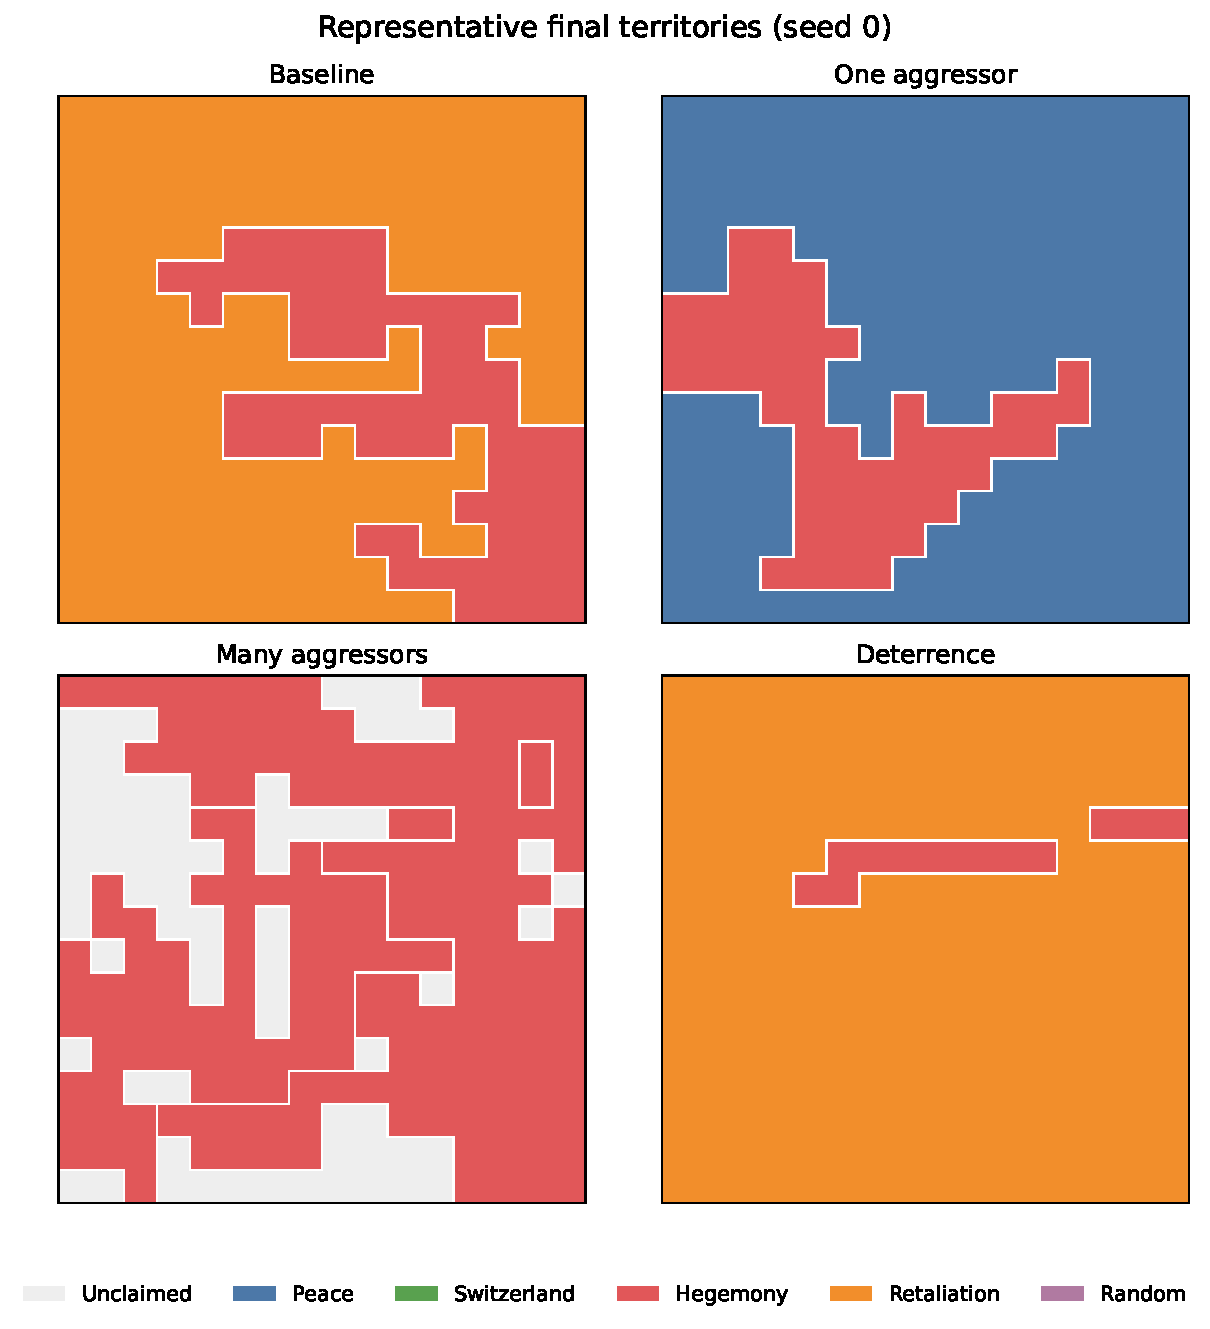
\includegraphics[width=0.94\textwidth]{../results/figures/01_final_maps.pdf}
\caption{Representative final territories for seed 0.  Colours identify
strategies; white cells are unclaimed.  These maps illustrate possible
outcomes, whereas quantitative conclusions use all 100 seeds.}
\label{fig:maps}
\end{figure*}

The baseline time series in Figure~\ref{fig:dynamics} clarifies the feedback
between population and territory.  Initial expansion increases carrying
capacity and population.  Once borders meet, attacks and pacts alter the
balance, and eliminated countries disappear from the trajectories.  Territory
changes discretely, while population responds gradually through growth,
famine, assimilation, and casualties.

\begin{figure*}[!t]
\centering
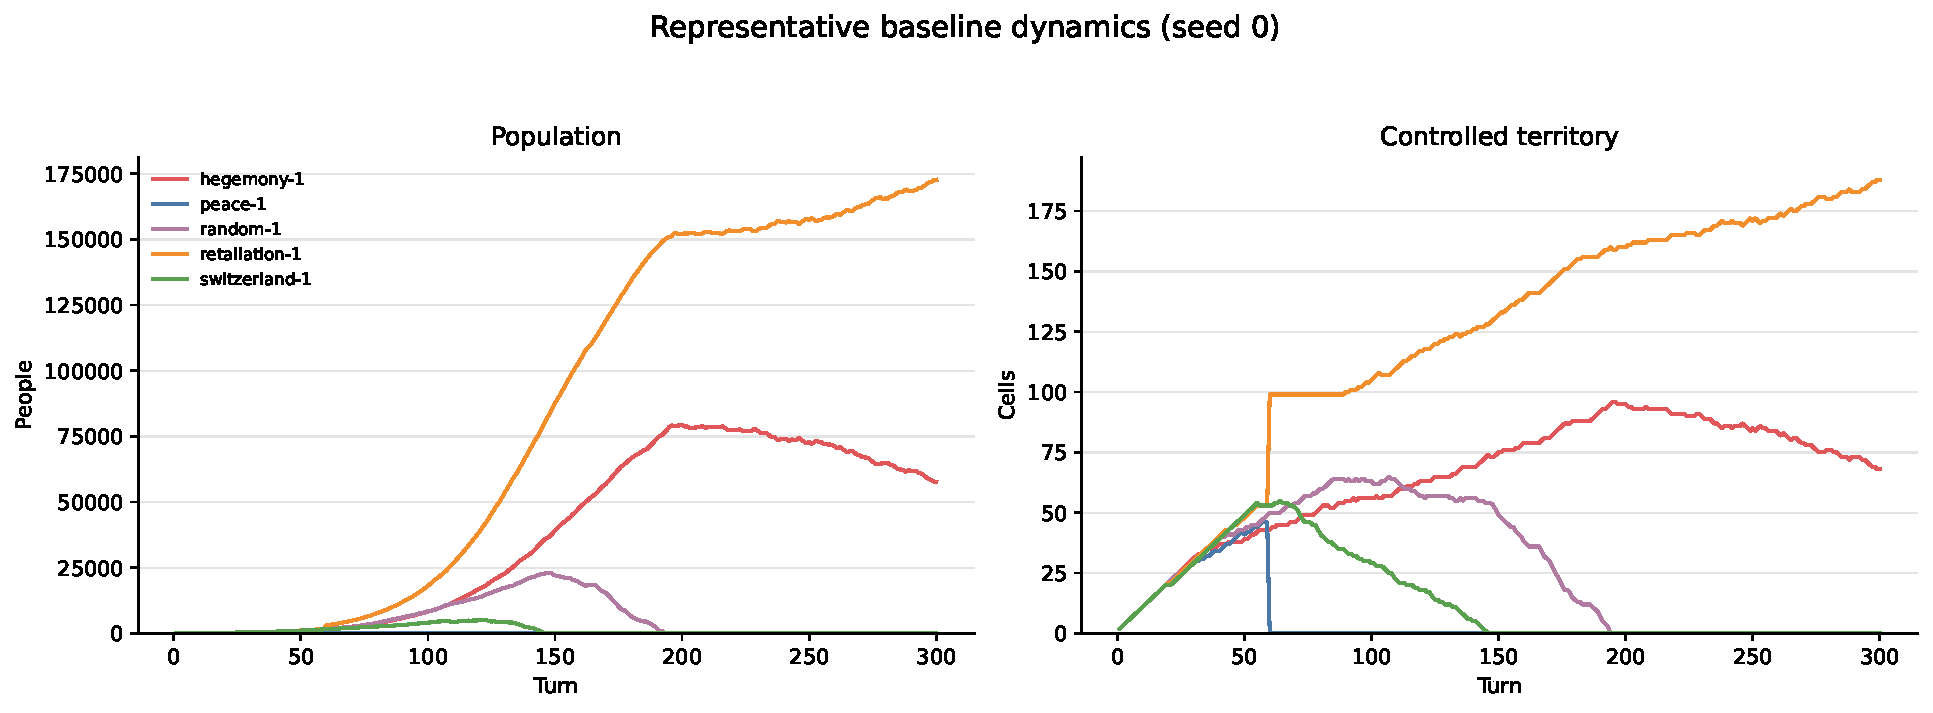
\includegraphics[width=0.94\textwidth]{../results/figures/06_sample_dynamics.pdf}
\caption{Representative country population and controlled-territory dynamics
in the baseline run (seed 0).  The figure is descriptive of one trajectory.}
\label{fig:dynamics}
\end{figure*}

\subsection{Baseline comparison}

Hegemony performs best on all three baseline outcome measures
(Table~\ref{tab:baseline} and Figure~\ref{fig:baseline}).  It survives 85\%
of runs, is dominant in 39\%, and controls 95.1 cells on average.  Retaliation
is second: 58\% survival, 29\% dominance, and 69.3 cells.  Random behaviour is
occasionally dominant but unstable; its median final population is zero.
Peace survives in 40\% of runs and dominates only 7\%.  Switzerland avoids
offensive casualties but is never dominant in the baseline and controls only
16.4 cells on average.  Thus, unconditional non-aggression does not protect a
country when an expansionist neighbour is present.

\begin{table}[t]
\centering
\caption{Baseline outcomes over 100 seeds.  Territory is the mean number of
cells at the end of a run.}
\label{tab:baseline}
\begin{tabular}{lrrr}
\toprule
Strategy & Survive & Dominant & Territory \\
\midrule
\strategy{Hegemony}    & 85\% & 39\% & 95.1 \\
\strategy{Retaliation} & 58\% & 29\% & 69.3 \\
\strategy{Random}      & 31\% & 25\% & 39.3 \\
\strategy{Peace}       & 40\% &  7\% & 34.9 \\
\strategy{Switzerland} & 47\% &  0\% & 16.4 \\
\bottomrule
\end{tabular}
\end{table}

\begin{figure*}[!t]
\centering
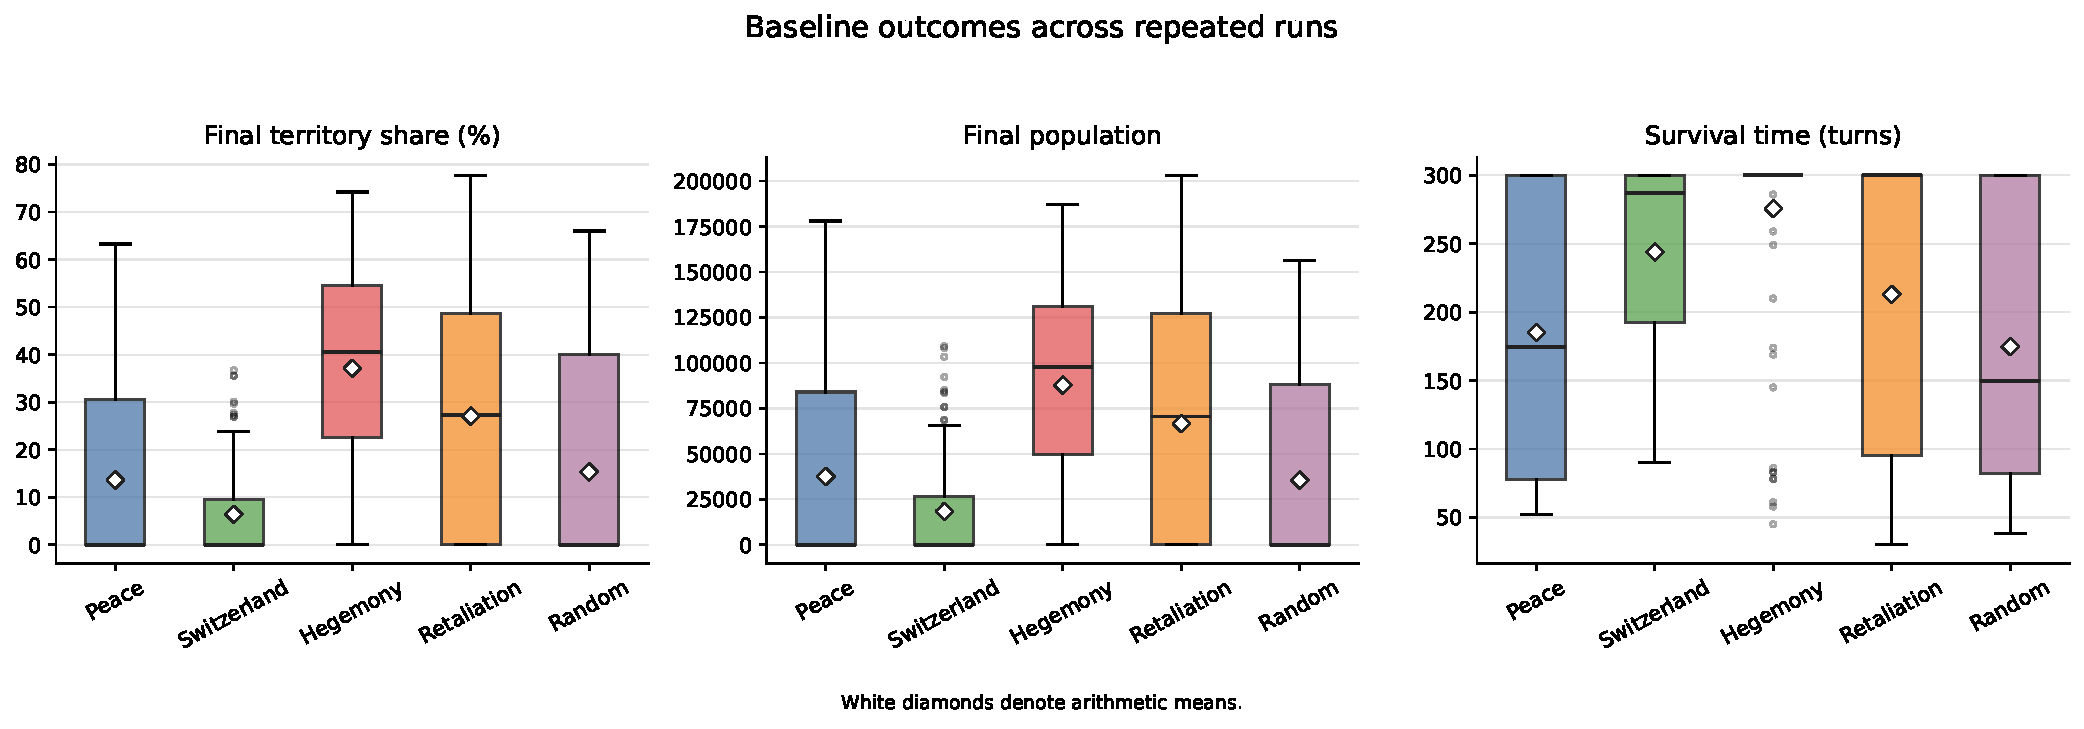
\includegraphics[width=0.94\textwidth]{../results/figures/02_baseline_outcomes.pdf}
\caption{Distributions of final territory, final population, and survival
time in the baseline scenario.  Each box summarizes 100 country outcomes;
white diamonds mark arithmetic means.}
\label{fig:baseline}
\end{figure*}

\subsection{Environmental conditions}

Figure~\ref{fig:heatmaps} compares the six common-composition environments.
Crowding is destructive for every strategy.  On the $8\times8$ map,
hegemony is dominant in 45\% of runs, while the other strategies have only
5--24\% dominance.  With abundant space, however, survival becomes common:
Switzerland reaches 99\%, hegemony 92\%, random 73\%, and retaliation 68\%.
Retaliation is dominant in 49\% of spacious runs, compared with only 2\% for
hegemony.  More land delays contact and permits populations to grow before
conflict; the retaliator then has both resources and a credible response.

\begin{figure*}[!t]
\centering
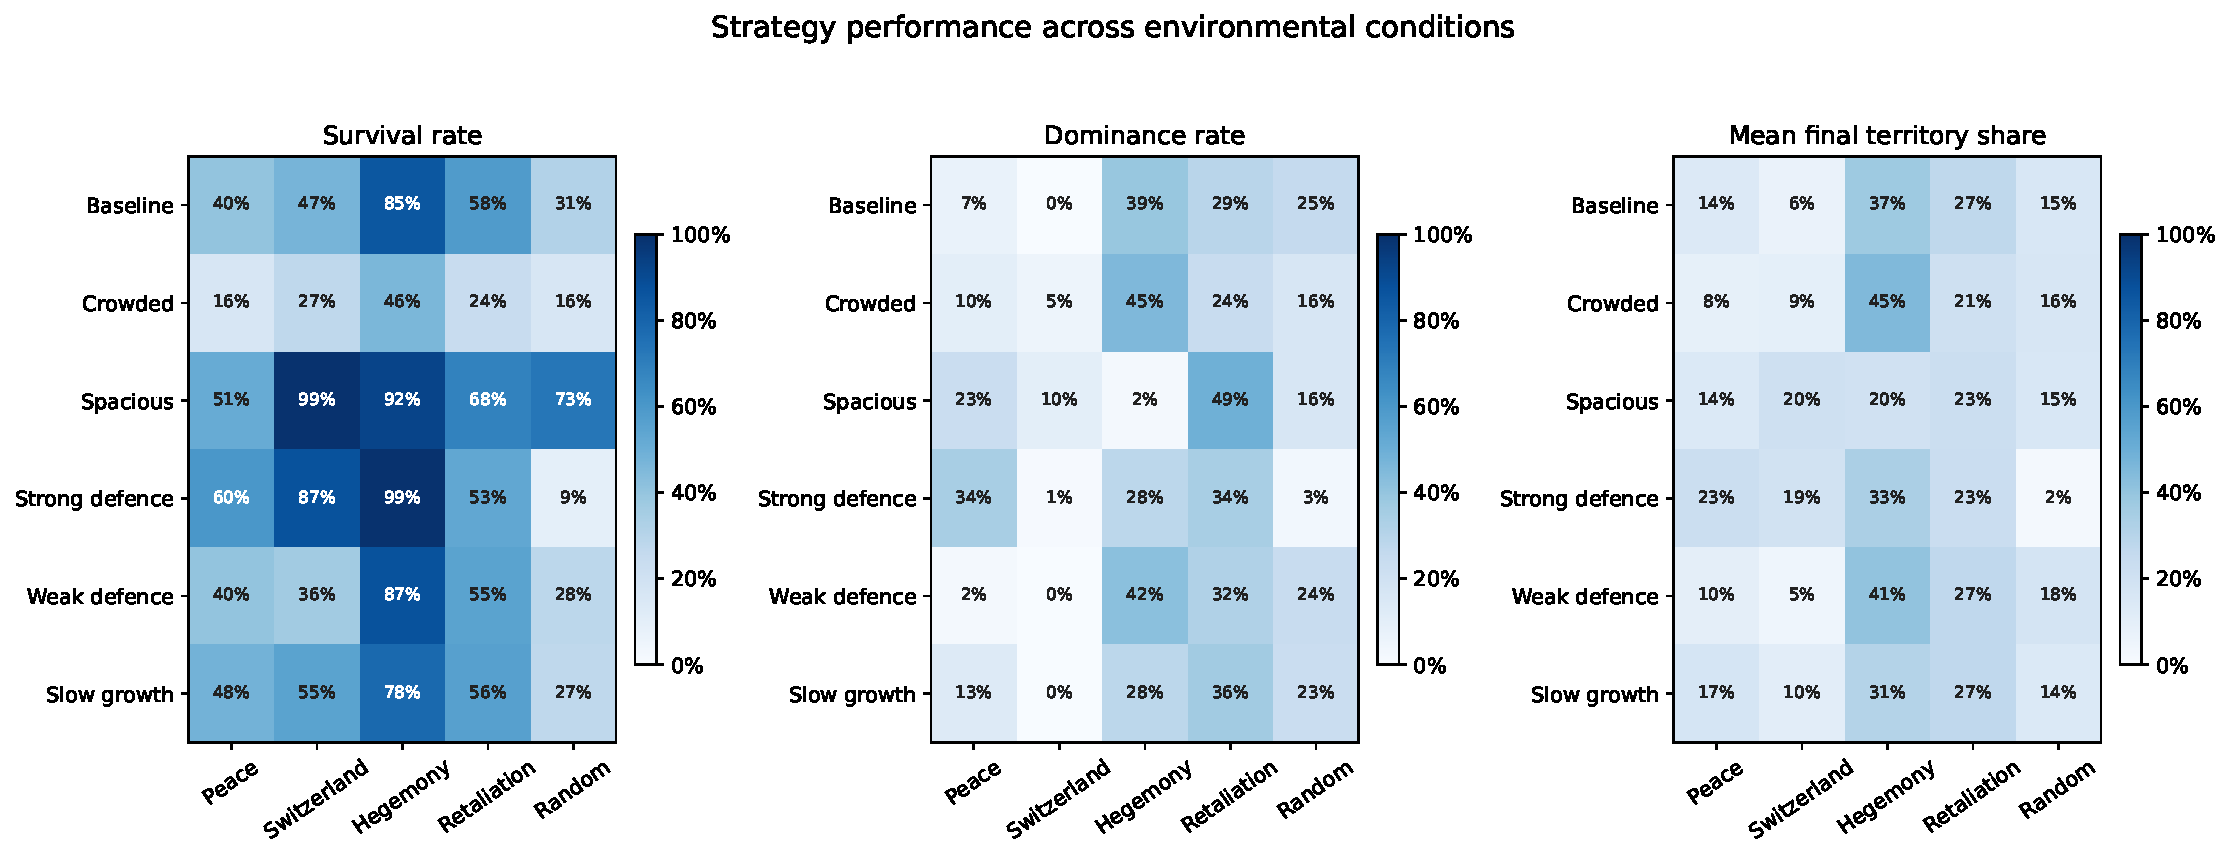
\includegraphics[width=0.94\textwidth]{../results/figures/03_scenario_heatmaps.pdf}
\caption{Mean survival, dominance, and final territory share by strategy
across six environmental conditions.  Each cell summarizes 100 runs.}
\label{fig:heatmaps}
\end{figure*}

Defence changes which strategies can convert survival into dominance.  At
$d=3$, hegemony still survives in 99\% of runs, but its dominance falls to
28\%; peace and retaliation each reach 34\% dominance.  Switzerland survives
87\% but dominates only 1\%, showing that survival and expansion are distinct
objectives.  Random behaviour collapses to 9\% survival because indiscriminate
attacks become expensive.  With no defender advantage ($d=1$), hegemony
controls 104.0 cells on average and dominates 42\% of runs.

The continuous sweeps in Figure~\ref{fig:sweeps} confirm these patterns using
territory share, which remains comparable as the map changes size.  From map
width 8 to 26, hegemony falls from 44.9\% to 19.7\% of the map, while
retaliation rises from 20.9\% to 22.5\% and Switzerland from 9.2\% to 20.5\%.
Increasing defence from 1 to 3 reduces hegemony from 40.6\% to 33.4\%, while
peace rises from 9.7\% to 22.6\% and Switzerland from 4.5\% to 18.8\%.
Faster growth benefits hegemony (30.8\% at $r=0.02$ versus 40.4\% at
$r=0.10$) but slightly harms peace and Switzerland, because it replenishes
the populations used to project military force as well as peaceful
populations.

\begin{figure*}[!t]
\centering
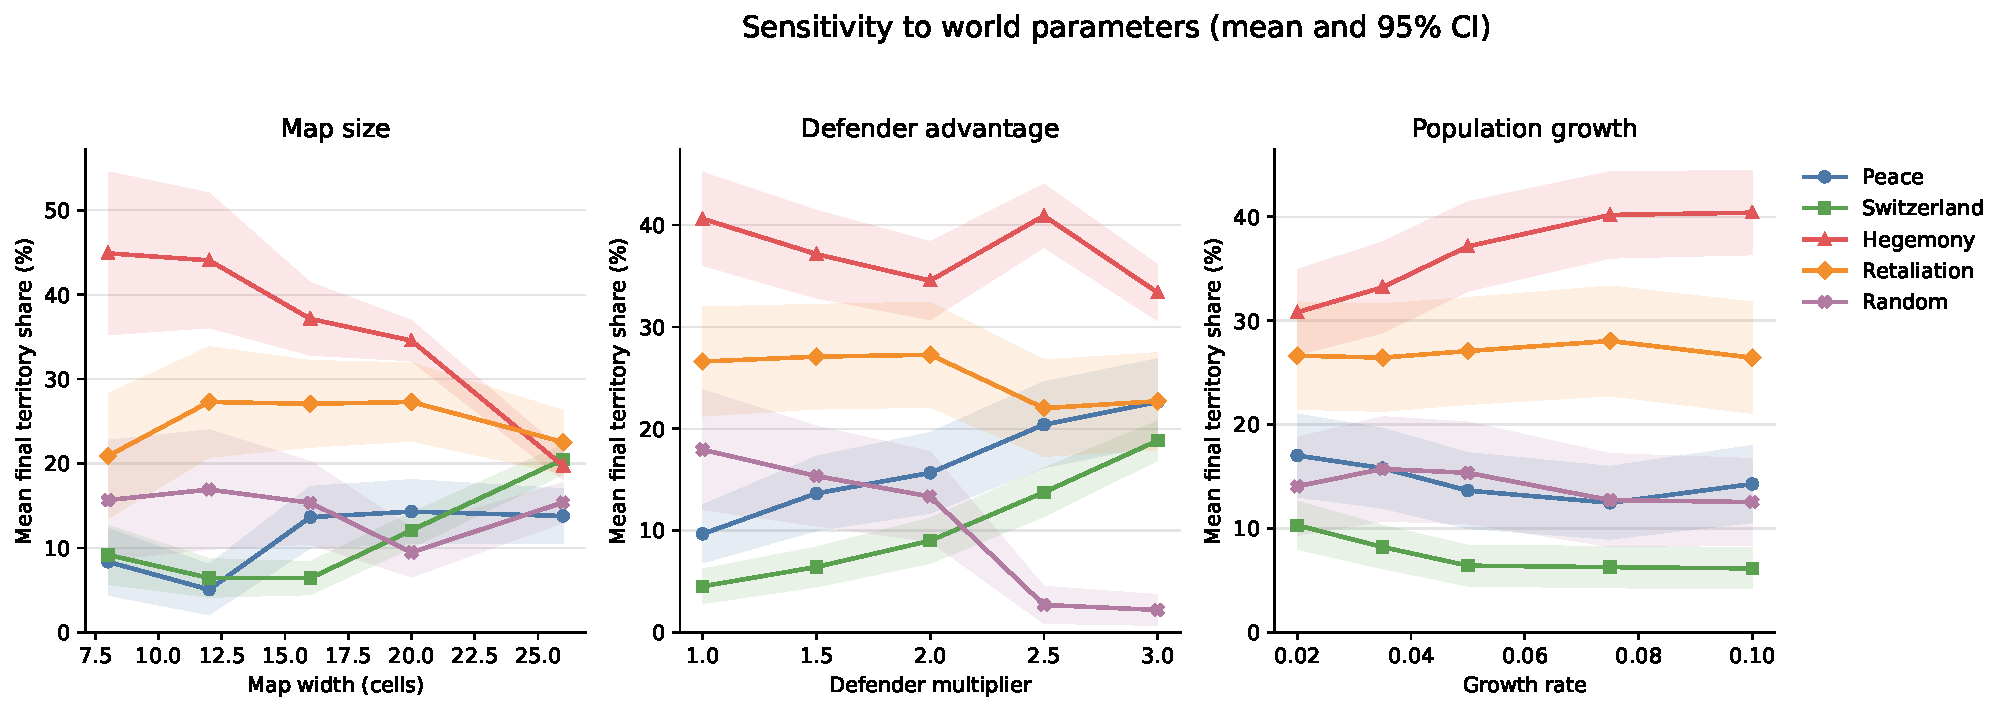
\includegraphics[width=0.94\textwidth]{../results/figures/04_parameter_sweeps.pdf}
\caption{Mean final territory share and 95\% Monte Carlo intervals under
map-width, defence-multiplier, and population-growth sweeps.  Only the
parameter on the horizontal axis changes within each panel.}
\label{fig:sweeps}
\end{figure*}

\subsection{Strategic context}

Performance changes sharply when the mix of neighbours changes
(Figure~\ref{fig:context}).  A single hegemony among four peaceful countries
survives every run, but the four peaceful countries collectively account for
almost all dominance: an individual peace country is dominant in 24.7\% of
its 400 observations, whereas the hegemony is dominant in only 1\% of runs.
The aggressor attacks early, but cooperation and occasional unions allow a
peaceful country to become the largest successor.

When four hegemonies compete, only 44\% survive and each makes 158 attacks on
average.  The single peace country survives only 19\%.  In the deterrence
scenario, retaliation is dominant in 31\% of observations and controls 64.7
cells on average, compared with 12.5\% and 38.5 cells for hegemony.  Retaliation
therefore changes the payoff of aggression: it does not eliminate attacks,
but it prevents aggressors from converting them into the same territorial
advantage.  In the neutral comparison, hegemony remains strongest; peace
survives slightly more often than Switzerland (41.5\% versus 38.0\%), partly
because peace can enter military alliances while Switzerland refuses them.

\begin{figure*}[!t]
\centering
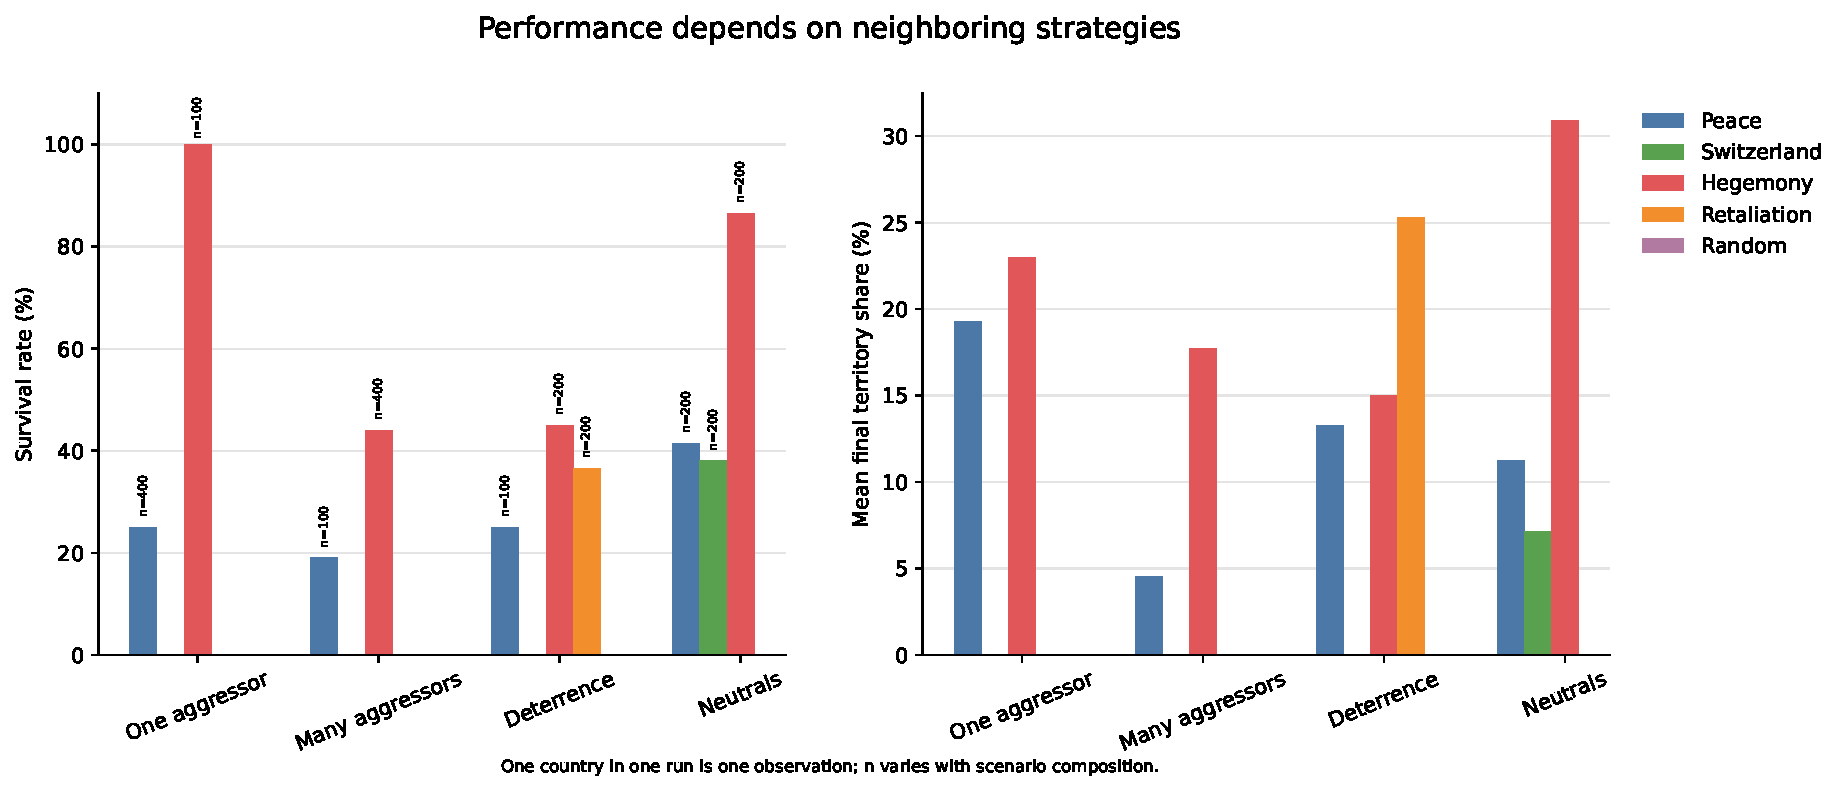
\includegraphics[width=0.94\textwidth]{../results/figures/05_strategic_context.pdf}
\caption{Outcomes under four changes in strategic composition.  Labels give
the number of observations for each strategy; repeated strategies contribute
multiple country observations per seed.}
\label{fig:context}
\end{figure*}

\section{Discussion}

\subsection{What does a group strategy mainly depend on?}

The experiments support four answers.  First, strategy depends on
\emph{resource pressure}.  On a crowded map, early contact makes conquest and
elimination frequent, strongly favouring hegemony.  On a spacious map,
countries can grow before meeting, and retaliation becomes more effective
than unconditional aggression.

Second, strategy depends on the \emph{relative price of attack}.  A high
defence multiplier protects peaceful and neutral countries and punishes the
random strategy's unnecessary wars.  This is not equivalent to removing
conflict: hegemony still survives, but it is less often the largest country.

Third, strategy depends on \emph{population recovery}.  Fast growth supplies
people for both production and combat.  In this model, aggressive countries
convert the additional population into territorial gains more effectively,
whereas slow growth makes casualties persistent.

Fourth, and most strongly, strategy depends on \emph{who the neighbours are}.
Hegemony exploits unconditional pacifism, yet multiple hegemonies impose large
costs on each other.  Retaliation is weak enough to avoid initiating war but
strong enough to alter an aggressor's expected gain.  Peace can outperform
armed neutrality when alliances and unions are valuable.  Consequently,
``best strategy'' is not a property of a strategy alone; it is a conditional
property of the spatial, military, demographic, and strategic environment.

These findings should be interpreted mechanistically rather than normatively.
Hegemony's strong baseline result follows from the chosen objective measures
and rules: territory raises carrying capacity, and conquest assimilates half
of a captured cell's population.  A welfare measure including total deaths,
inequality, or pact stability would rank strategies differently.  The model
therefore demonstrates how assumptions and outcome definitions shape a
strategic conclusion.

\section{Limitations}

The model intentionally favours clarity over realism.  Its main limitations
are the following.

\begin{itemize}
\item The assignment proposes providers, warriors, and scientists whose roles
can change.  The implementation instead aggregates all members into one
population.  Technology, labour allocation, and internal adaptation are not
modelled; adding them is the most important extension.
\item Every cell has equal productivity.  The proposed non-uniform resource
landscape, food stocks, transfers during scarcity, terrain, travel costs, and
capitals are absent.  Trade is represented only as a carrying-capacity bonus.
\item Countries expand through adjacent cells, but the model does not enforce
that a defender's remaining cells stay connected after conquest.  Fragmented
territory can therefore occur.
\item One country takes one action per turn regardless of population or area.
Large states do not have proportionally more administrative or military
actions.
\item Strategies are fixed, transparent to the experimenter, and incapable
of learning.  Countries cannot change doctrine, infer an opponent's strategy,
or negotiate contingent agreements.
\item Parameter values are illustrative rather than calibrated to empirical
human-group data.  Results establish behaviour of this model, not causal
claims about real societies.
\item Only one-factor sweeps are reported.  Interactions between map size,
defence, growth, and composition may be nonlinear and require a factorial or
global sensitivity analysis.
\item Monte Carlo uncertainty reflects seed-to-seed variability only.  It
does not capture structural uncertainty in the model rules.
\end{itemize}

\section{Conclusions}

This project implements a reproducible agent-based simulation of territorial
human groups and evaluates five strategies over 2,500 stochastic runs.
Aggressive hegemony is the strongest strategy under the baseline assumptions,
but its advantage is neither universal nor synonymous with survival.
Retaliation becomes the leading strategy when land is abundant or when it
directly confronts aggressors.  Strong defence makes peaceful cooperation
competitive, while neutrality protects survival more reliably than dominance.

The principal conclusion is therefore conditional: a group's success depends
on resource scarcity, the defensive advantage, demographic recovery, and the
strategies of neighbouring groups.  The separation of data collection from
plotting, fixed seeds, run-level outputs, and automated checks make these
claims reproducible.  Extending the model with explicit providers, warriors,
scientists, heterogeneous resources, and adaptive strategies would allow the
next study to address the full internal-group dynamics proposed in the
original project description.

\begin{thebibliography}{9}

\bibitem{bonabeau2002}
E. Bonabeau,
``Agent-based modeling: Methods and techniques for simulating human systems,''
\emph{Proceedings of the National Academy of Sciences}, vol. 99, suppl. 3,
pp. 7280--7287, 2002.
\href{https://doi.org/10.1073/pnas.082080899}{doi:10.1073/pnas.082080899}.

\bibitem{schelling1971}
T. C. Schelling,
``Dynamic models of segregation,''
\emph{Journal of Mathematical Sociology}, vol. 1, no. 2, pp. 143--186, 1971.
\href{https://doi.org/10.1080/0022250X.1971.9989794}{doi:10.1080/0022250X.1971.9989794}.

\bibitem{epstein1996}
J. M. Epstein and R. L. Axtell,
\emph{Growing Artificial Societies: Social Science from the Bottom Up}.
Washington, DC: Brookings Institution Press and MIT Press, 1996.

\bibitem{axelrod1981}
R. Axelrod and W. D. Hamilton,
``The evolution of cooperation,''
\emph{Science}, vol. 211, no. 4489, pp. 1390--1396, 1981.
\href{https://doi.org/10.1126/science.7466396}{doi:10.1126/science.7466396}.

\end{thebibliography}

\end{document}
